\documentclass[unicode]{beamer}

\usepackage[orientation=landscape,size=a0,scale=1.4]{beamerposter}
\usepackage{booktabs}
\usepackage{graphicx}

\usepackage{tikz}
\usetikzlibrary{
  arrows.meta, % for changing arrow head size
}

\setbeamercolor{hokudai}{bg=hokudai!20}

\usetheme[footertext={
  27th International Conference on Pattern Recognition, December 01--05, 2024,
  Kolkata, India
  }]{SimplePoster}

\title{
  R-LIME:\ Rectangular Constraints and Optimization for
  Local Interpretable Model-agnostic Explanation Methods
}

\begin{document}
\begin{frame}
	\begin{columns}[t]
		\def\lcol{0.43}
		\def\rcol{0.53}
		\begin{column}{\lcol\linewidth}
			\begin{block}{LIME \Large(Local Interpretable Model-agnostic Explanations)}
				\begin{columns}
					\begin{column}{.65\textwidth}
						{
							\renewcommand{\leftmargini}{2.5em}
							\begin{enumerate}
								\item Sample perturbed instances around the given focal point
								\item Learn a linear model on the instances
							\end{enumerate}
						}
					\end{column}
					\begin{column}{.35\textwidth}
						\begin{figure}
							\centering
							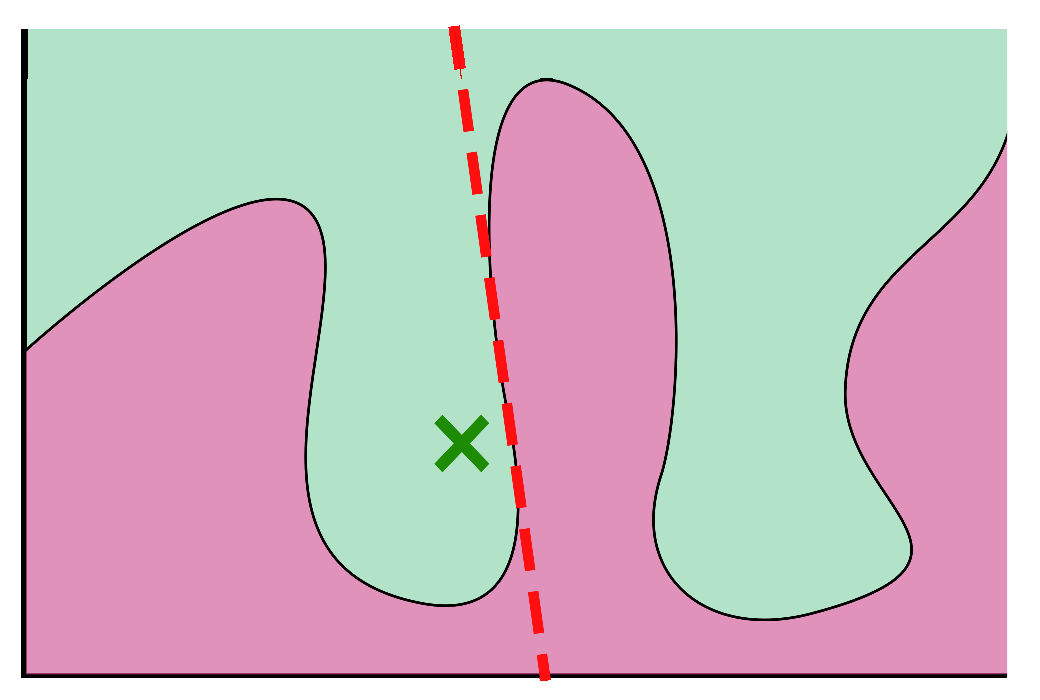
\includegraphics[width=.8\textwidth]{src/img/visual-lime}
						\end{figure}
					\end{column}
				\end{columns}
			\end{block}
			\begin{block}{Anchor}
				\begin{columns}
					\begin{column}{.65\textwidth}
						{
							\renewcommand{\leftmargini}{2.5em}
							\begin{enumerate}
								\item Maximize the rectangular region as long as
								      the model’s outputs are consistent with high probability
							\end{enumerate}
						}
					\end{column}
					\begin{column}{.35\textwidth}
						\begin{figure}
							\centering
							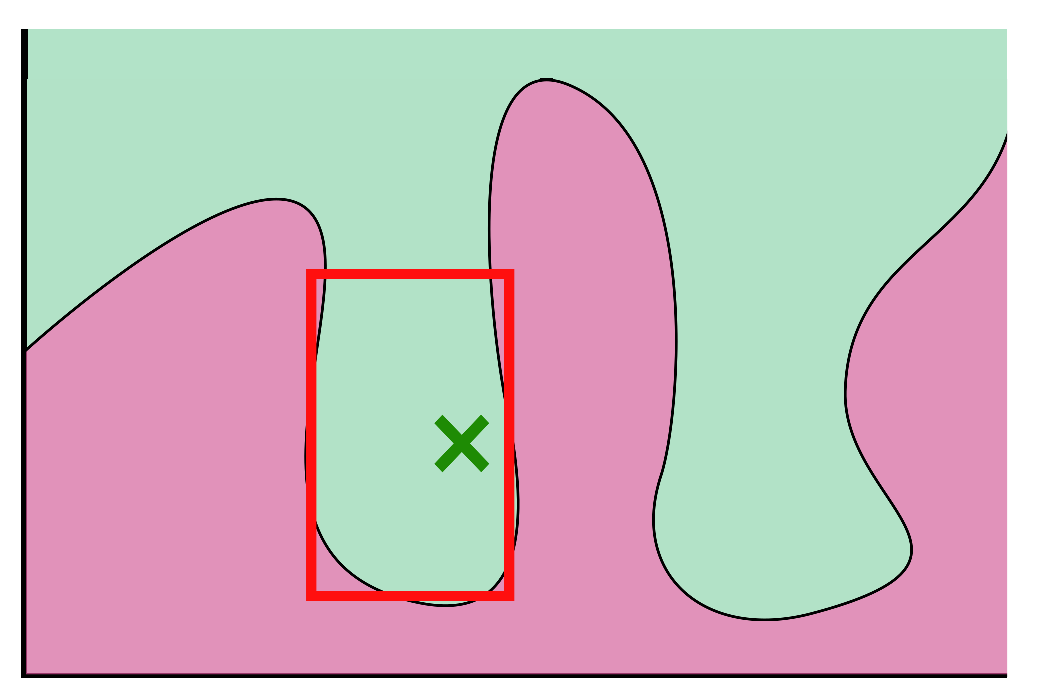
\includegraphics[width=.8\textwidth]{src/img/visual-anchor}
						\end{figure}
					\end{column}
				\end{columns}
			\end{block}
		\end{column}
		\begin{column}{\rcol\linewidth}%
			\begin{block}{Our Method: R-LIME (Ruled LIME)}
				\hspace{0px}
				\begin{beamercolorbox}[wd=.35\textwidth,colsep=.4em,rounded=true,shadow=true]{hokudai}
					\textbf{R-LIME} = LIME + Anchor
				\end{beamercolorbox}
				\vspace{.2em}
				\begin{columns}
					\begin{column}{0.66\textwidth}
						\begin{itemize}
							\item Approximate in rectangular region
							\item Maximize the region as long as approximation accuracy is
							      higher than the given threshold
							\item Express the region as a conjunction of feature predicates \\[0.5em]
						\end{itemize}
					\end{column}
					\begin{column}{0.27\textwidth}
						\begin{figure}
							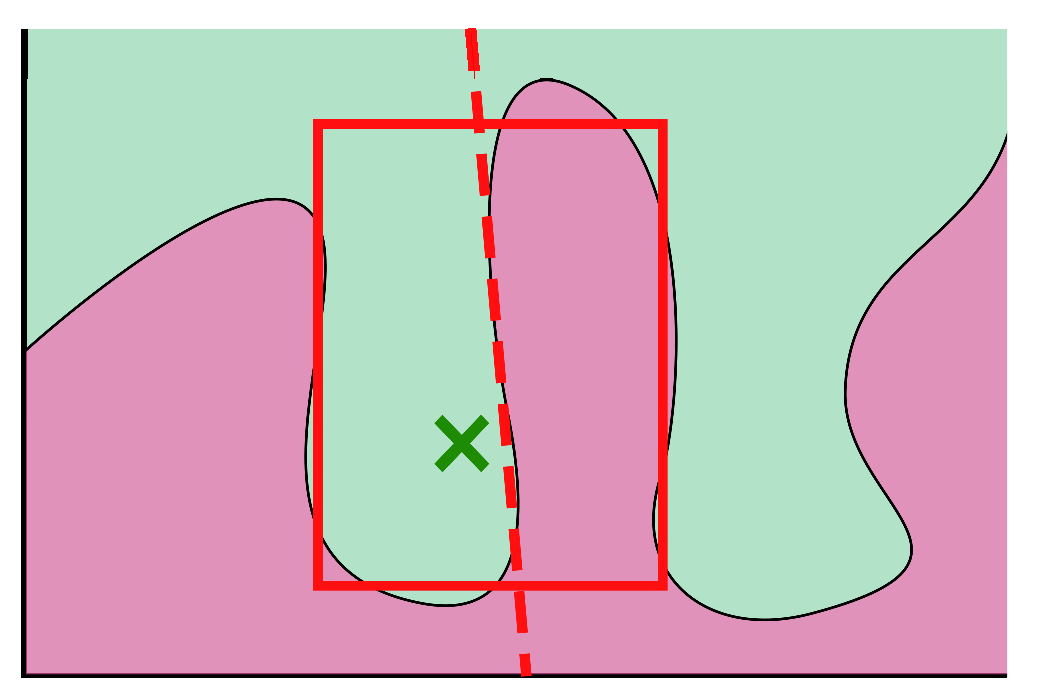
\includegraphics[width=\textwidth]{src/img/visual-rlime3}
						\end{figure}
					\end{column}
				\end{columns}
				\vspace{1.25em}
				\begin{columns}
					\centering
					\begin{column}{.22\textwidth}
						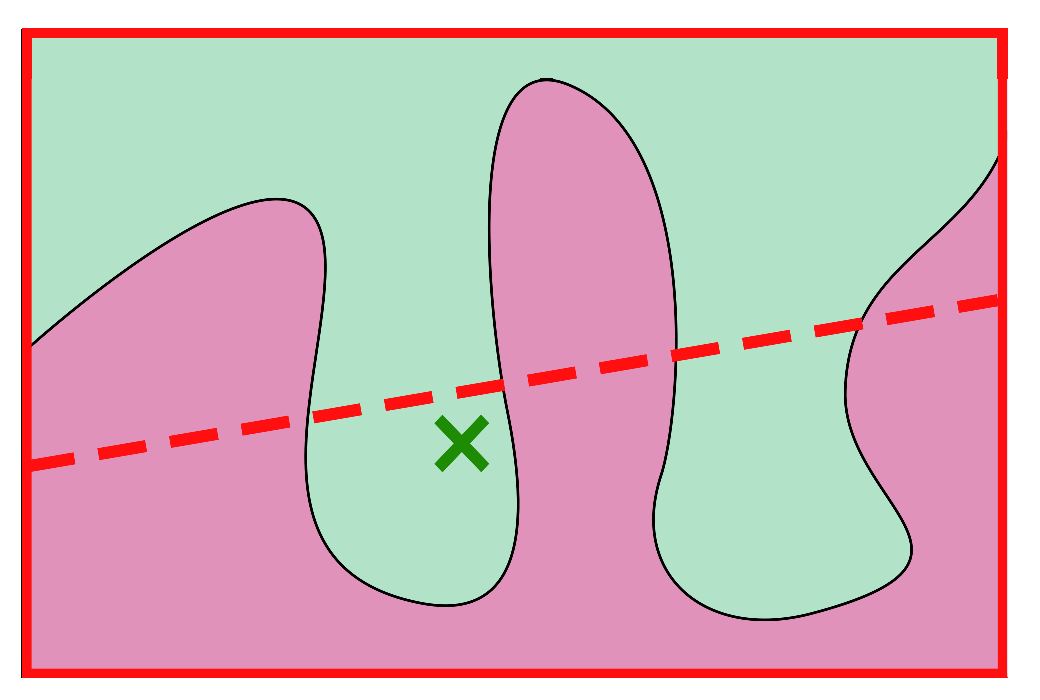
\includegraphics[width=\textwidth]{src/img/visual-rlime1}
					\end{column}
					\begin{column}{.05\textwidth}
						\begin{center}
							\begin{tikzpicture}
								\draw [-{Latex[length=3mm, width=4mm]}] (0,-10) -- (3, -10);
							\end{tikzpicture}
						\end{center}
					\end{column}
					\begin{column}{.22\textwidth}
						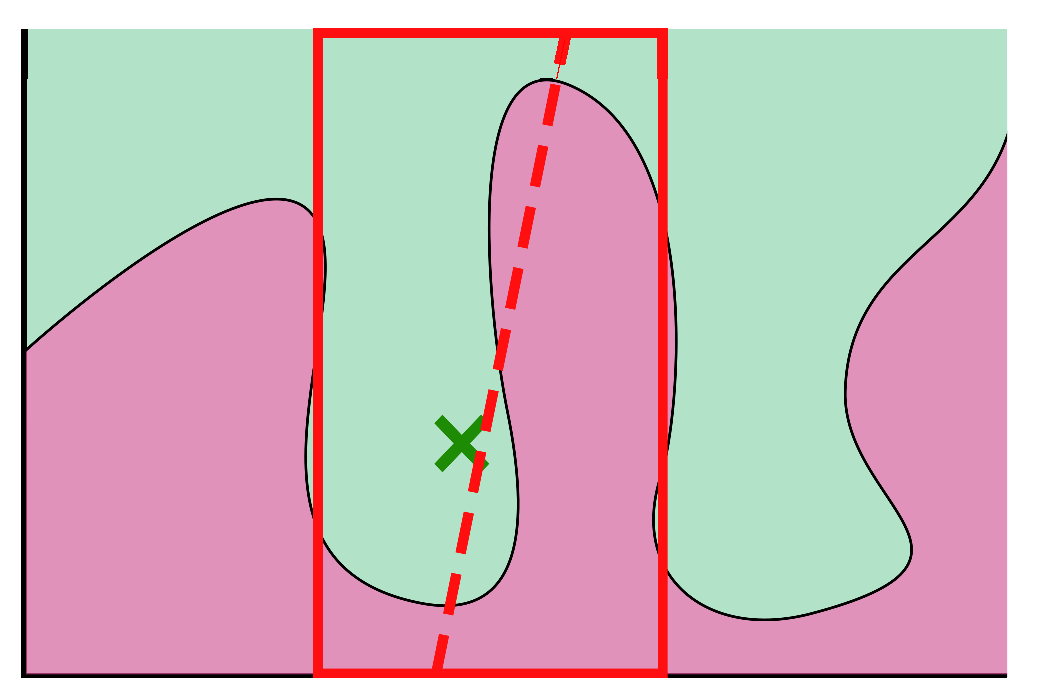
\includegraphics[width=\textwidth]{src/img/visual-rlime2}
					\end{column}
					\begin{column}{.05\textwidth}
						\begin{center}
							\begin{tikzpicture}
								\draw [-{Latex[length=3mm, width=4mm]}] (0,-10) -- (3, -10);
							\end{tikzpicture}
						\end{center}
					\end{column}
					\begin{column}{.22\textwidth}
						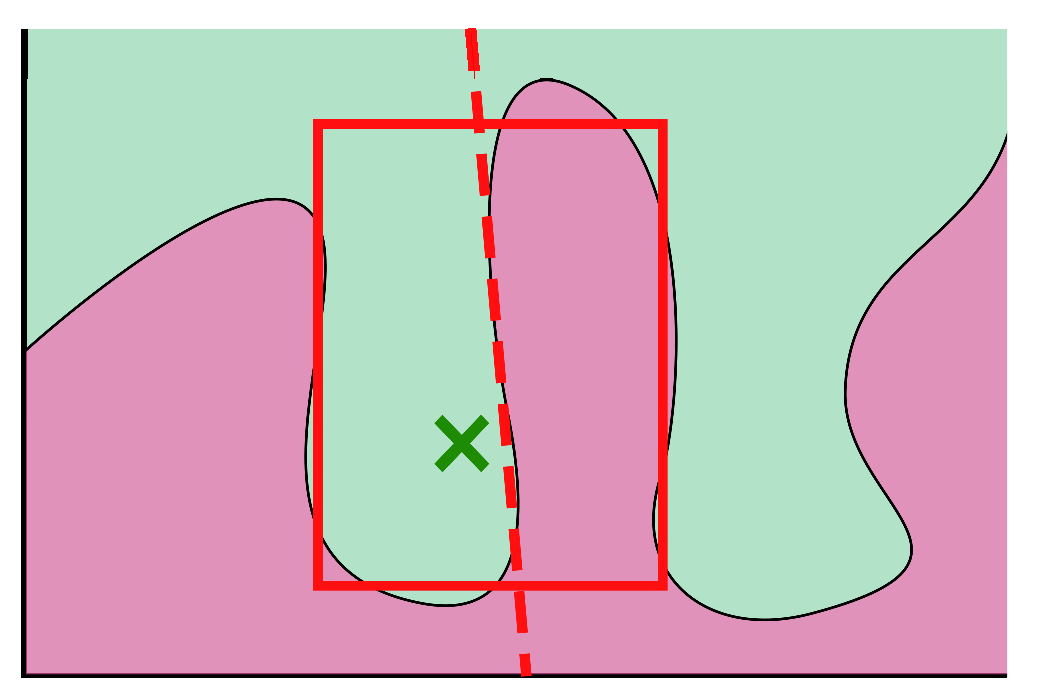
\includegraphics[width=\textwidth]{src/img/visual-rlime3}
					\end{column}
				\end{columns}
			\end{block}
		\end{column}
	\end{columns}
	\vspace{.8em}
	\begin{columns}[t]
		\begin{column}{.97\linewidth}
			\begin{block}{LIME vs. Anchor vs. R-LIME}
				\begin{columns}
					\def\lcol{0.36}
					\def\ccol{0.23}
					\def\rcol{0.38}
					\begin{column}{\lcol\textwidth}
						\def\lcol{0.5}
						\def\rcol{0.45}
						\begin{columns}[]
							\begin{column}{\lcol\textwidth}
								\begin{figure}
									
\includegraphics[width=\textwidth]{src/img/example-instance}

									\vspace{-0.3em}
									\caption{The focal point}
								\end{figure}
								\vspace{0.5em}
								\begin{figure}
									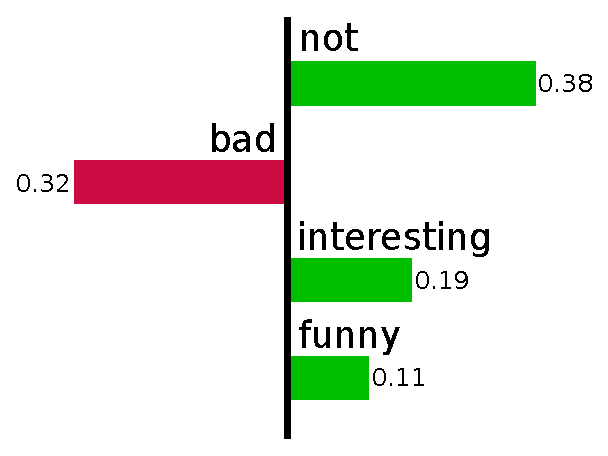
\includegraphics[width=\textwidth]{src/img/example-lime}
									\caption{LIME's explanation}
								\end{figure}
								\vspace{0.5em}
								\begin{figure}
									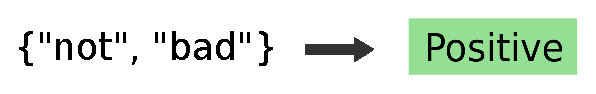
\includegraphics[width=\textwidth]{src/img/example-anchor}

									\vspace{-0.3em}
									\caption{Anchor's explanation}
								\end{figure}
							\end{column}
							\begin{column}{\rcol\textwidth}
								\begin{figure}
									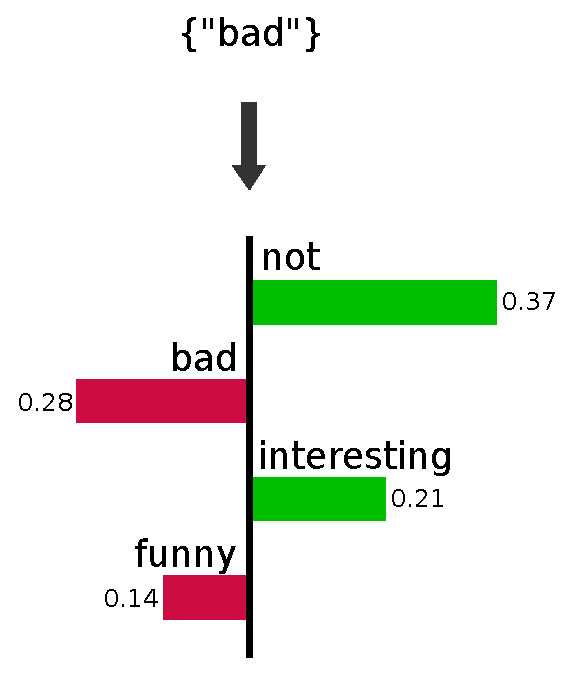
\includegraphics[width=\textwidth]{src/img/example-rlime}
									\caption{R-LIME's explanation}
								\end{figure}
							\end{column}
						\end{columns}
					\end{column}
					\vrule{}
					\begin{column}{\ccol\textwidth}
						\vspace{-0.5em}
						\begin{figure}
							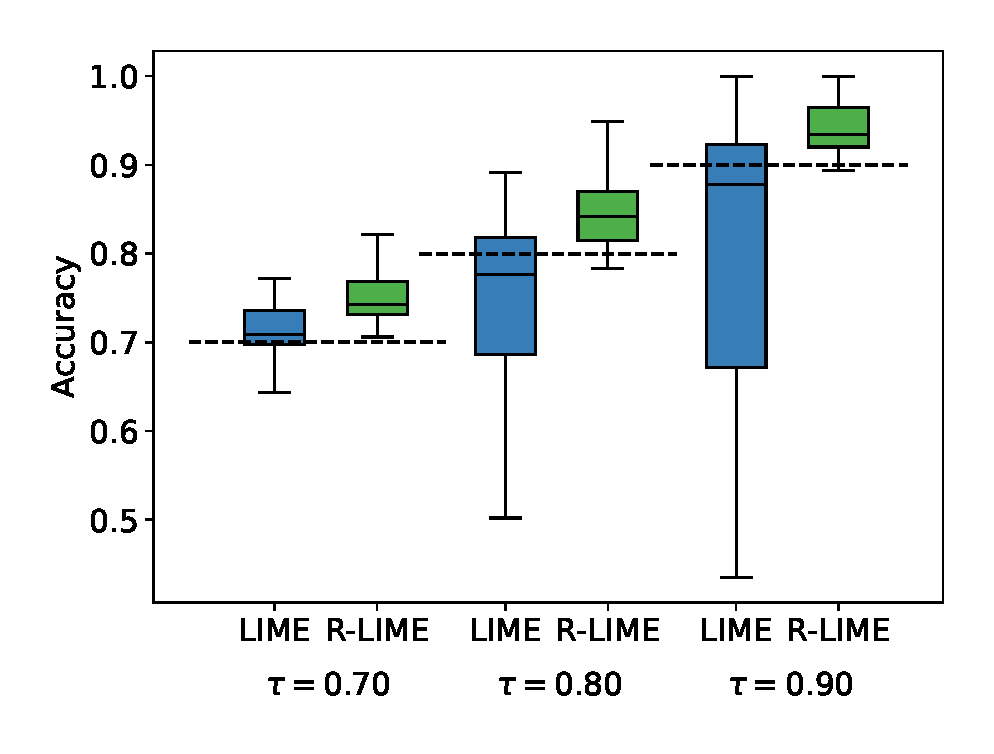
\includegraphics[width=.83\textwidth]{src/experiments/exp2/box_plot}
							\vspace{-1.0em}
							\caption{LIME vs. R-LIME (in accuracy)}
						\end{figure}
						\begin{figure}
							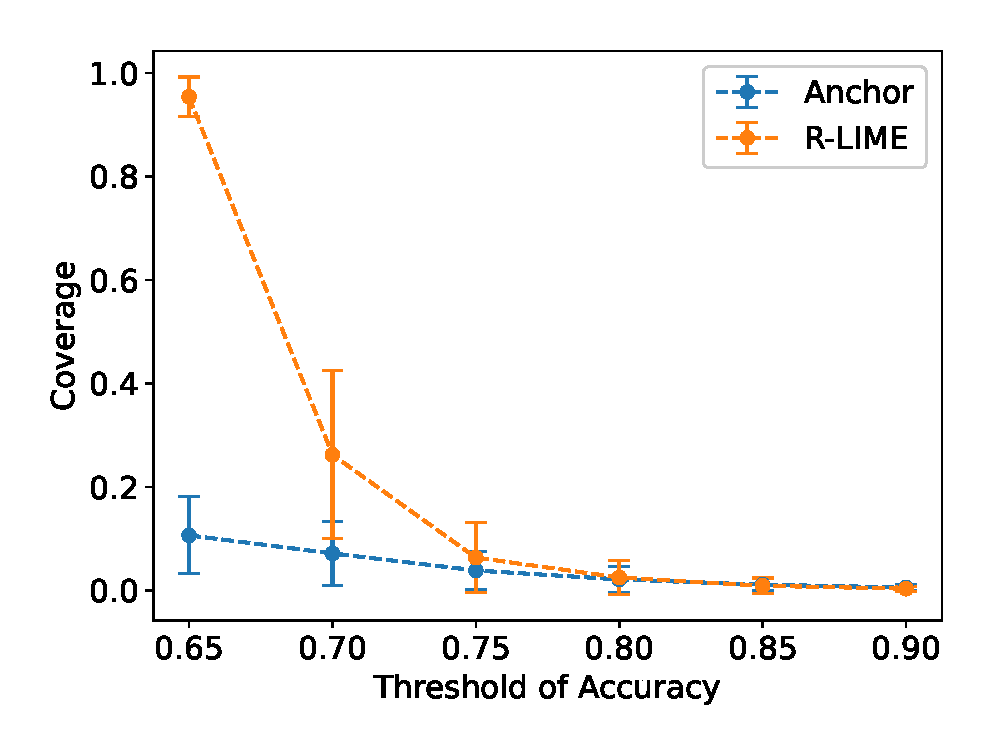
\includegraphics[width=.83\textwidth]{src/experiments/exp2/comp_cov}
							\vspace{-1.0em}
							\caption{LIME vs. R-LIME (in coverage)}
						\end{figure}
					\end{column}
					\vrule{}
					\begin{column}{\rcol\textwidth}
						\renewcommand{\arraystretch}{1.3}
						\tabcolsep=0.6em
						\begin{center}
							\begin{tabular}{cccc}
								                    & LIME         & Anchor       & \textbf{R-LIME} \\
								\midrule
								Feature Importance  & \checkmark{} & $\times$     & \checkmark{}    \\
								Optimal Scope       & $\times$     & \checkmark{} & \checkmark{}    \\
								Interpretable Scope & $\times$     & \checkmark{} & \checkmark{}    \\
							\end{tabular}
						\end{center}
						\vspace{1.5em}
						\begin{center}~%
							\begin{beamercolorbox}[wd=.9\textwidth,colsep=.5em,rounded=true,shadow=true]{hokudai}%
								\begin{itemize}
									\item Achieved interpretability of both explanation and its scope! \\ [0.8em]
									      Also:
									      \begin{itemize}
										      \Large
										      \item More accurate than LIME
										      \item More general than Anchor
									      \end{itemize}
								\end{itemize}
							\end{beamercolorbox}~%
						\end{center}
					\end{column}
				\end{columns}
			\end{block}
		\end{column}
	\end{columns}
\end{frame}

\end{document}
